\textbf{Ejemplo 4}\\
\vspace{2mm}
Un documento estipula pagos trimestrales de  800.000 COP durante 6 años. Si este documento se cancela con un solo pago de:

a) VP =  COP ? al principio; con una tasa del 24\% nominal anual trimestre vencido.\\
b) VF =  COP ? al final, con una tasa del 24\% nominal anual trimestre vencido.\\
%\newpage %USAR SOLO SI EL SOLUCIÓN QUEDA SOLO Y ES NECESARIO BAJARLO A LA SIGUIENTE PAGINA
\textbf{Solución.}\\
%La tabla ira centrada
\begin{center}
 \renewcommand{\arraystretch}{1.5}% Margenes de las celdas
 %Creación de la cuadricula de 3 columnas
 \begin{longtable}[H]{|p{0.333\linewidth}|p{0.3333\linewidth}|p{0.3333\linewidth}|}
  \hline
  \multicolumn{3}{|c|}{\cellcolor[HTML]{FFB183}\textbf{1. Declaración de variables}}                                  \\ \hline
  $R= 800.000 COP$         & $i=\frac{24\% \hspace{1mm} natv}{4 \hspace{1mm} ptv} = 6\% \hspace{1mm} ptv$ & $VP =  ?$ COP \\
  $n=24 \hspace{1mm} ptv$ &                                                                              & $VF=  ?$ COP   \\ \hline
  \multicolumn{3}{|c|}{\cellcolor[HTML]{FFB183}\textbf{2. Tabla de flujo de caja}}                                    \\ \hline
  \multicolumn{3}{|p{\columnwidth}|}{
  \begin{center}
   \begin{tabular}{|p{4cm}|p{4cm}|}
    \hline
    \textbf{Periodo (ptv)} & \textbf{Flujo} \\ \hline
    0                      &  COP  -           \\ \hline
    1                      &  800.000 COP    \\ \hline
    2                      &  800.000 COP    \\ \hline
    3                      &  800.000 COP    \\ \hline
    4                      &  800.000 COP    \\ \hline
    5                      &  800.000 COP    \\ \hline
    6                      &  800.000 COP    \\ \hline
    7                      &  800.000 COP    \\ \hline
    8                      &  800.000 COP    \\ \hline
    9                      &  800.000 COP    \\ \hline
    10                     &  800.000 COP    \\ \hline
    11                     &  800.000 COP    \\ \hline
    12                     &  800.000 COP    \\ \hline
    13                     &  800.000 COP    \\ \hline
    14                     &  800.000 COP    \\ \hline
    15                     &  800.000 COP    \\ \hline
    16                     &  800.000 COP    \\ \hline
    17                     &  800.000 COP    \\ \hline
    18                     &  800.000 COP    \\ \hline
    19                     &  800.000 COP    \\ \hline
    20                     &  800.000 COP    \\ \hline
    21                     &  800.000 COP    \\ \hline
    22                     &  800.000 COP    \\ \hline
    23                     &  800.000 COP    \\ \hline
    24                     &  800.000 COP    \\ \hline
   \end{tabular}
  \end{center}
  }                                                                                                                   \\ \hline
  \multicolumn{3}{|c|}{\cellcolor[HTML]{FFB183}\textbf{3. Fórmulas utilizadas}}                                       \\ \hline
  \multicolumn{3}{|p{\columnwidth}|}{Mediante el uso de Excel:
  \begin{itemize}
   \item VA (Valor actual): Devuelve el valor presente para una inversión
   \item VF (Valor Futuro): Devuelve el valor futuro de una inversión basado en pagos
         periódicos y constantes, y una tasa de interés constante
  \end{itemize}
  }                                                                                                                   \\ \hline
  \multicolumn{3}{|c|}{\cellcolor[HTML]{FFB183}\textbf{4. Desarrollo en Excel}}                                       \\ \hline
  \multicolumn{3}{|l|}{Se aplicará la función VA de la siguiente forma:}                                              \\
  \multicolumn{3}{|c|}{ 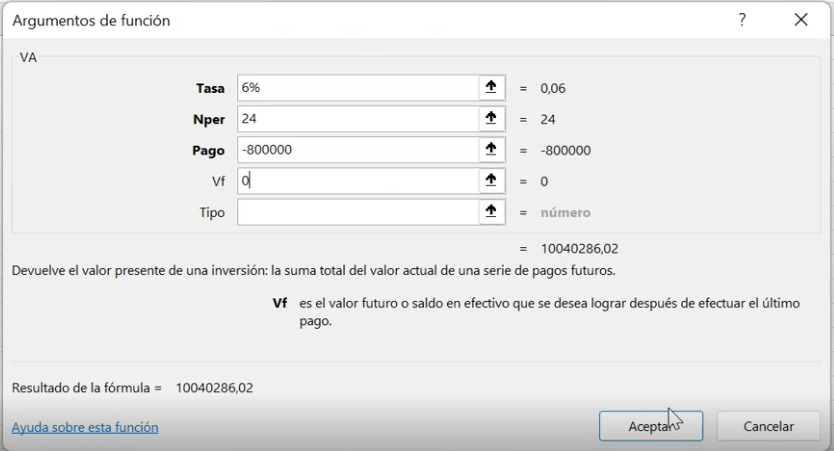
\includegraphics[trim=-5 -5 -5 -5 ,width=1\columnwidth]{4/Ejem4.1.png}}                        \\
  \multicolumn{3}{|l|}{E=VA(0,06;24;-800000) con referencia en la hoja de Excel usada para el ejercicio.}             \\
  \multicolumn{3}{|c|}{ 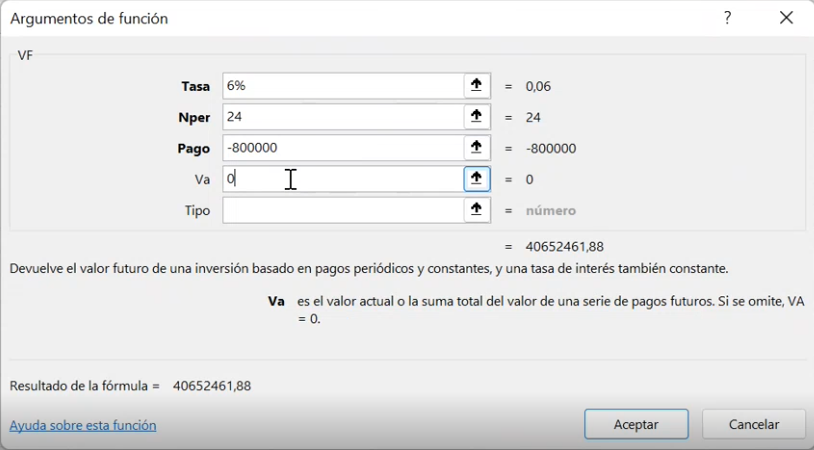
\includegraphics[trim=-5 -5 -5 -5 ,width=1\columnwidth]{4/Ejem4.2.png}}                        \\
  \multicolumn{3}{|l|}{ =VF(0,06;24;-800000) con referencia en la hoja de Excel usada para el ejercicio.}             \\ \hline
  \multicolumn{3}{|c|}{\cellcolor[HTML]{FFB183}\textbf{5. Respuesta}}                                                 \\ \hline
  \multicolumn{3}{|p{\columnwidth}|}{
  El valor presente (VP) o valor actual (VA) es $10.040.286 y el valor futuro (VF) es
  $40.652.461
  }                                                                                                                   \\ \hline
  \multicolumn{3}{|c|}{\cellcolor[HTML]{FFB183}\textbf{6. Gráfica}}                                                   \\ \hline
  \multicolumn{3}{|c|}{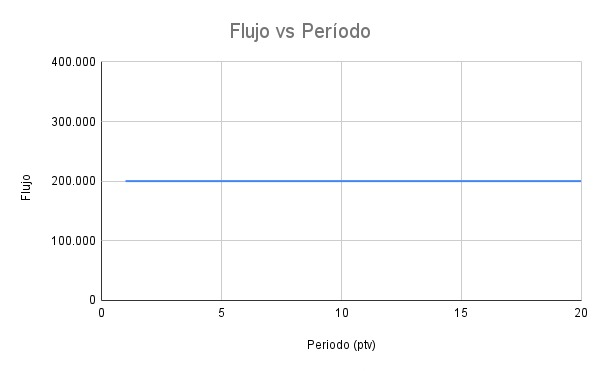
\includegraphics[trim=-5 -5 -5 -5 ,width=0.7\columnwidth]{4/flujovsperiodo.png}}                      \\ \hline
 \end{longtable}
 %\newline \newline %USARLO SI CREES QUE ES NECESARIO
\end{center}
